\chapter[Conformal Bootstrap and Modular Invariance]{Conformal Bootstrap and\\Modular Invariance}

In this chapter, we are going to discuss two deeply interconnected and remarkably powerful conceptual pillars of conformal field theory: the conformal bootstrap and modular invariance. The conformal bootstrap is a rigorous analytical method used to tightly constrain (and, in exactly solvable models, completely determine) the dynamical structure of CFTs by enforcing fundamental consistency conditions that arise from the operator product expansion (OPE) and crossing symmetry. Modular invariance, on the other hand, provides a macroscopic consistency requirement when the CFT is defined on a topologically non-trivial surface like the torus, allowing us to definitively classify the allowed operator content of minimal models.

\section{Conformal Bootstrap and Crossing Symmetry}

One of the most profound and revolutionary ideas in conformal field theory is that purely mathematical consistency conditions alone can strongly constrain, and in some cases completely determine, the full interacting dynamics of the theory.

The conformal bootstrap program is built mathematically upon three foundational ingredients:
\begin{itemize}
    \item \textbf{Global Conformal Symmetry:} which strictly dictates the coordinate dependence of two- and three-point functions, and restricts four-point functions to depend only on invariant cross-ratios.
    \item \textbf{The Operator Product Expansion (OPE):} which allows us to systematically replace the product of two nearby operators with an infinite sum of local operators.
    \item \textbf{Associativity of the OPE:} which physically translates to the statement that correlation functions must be uniquely defined and single-valued, regardless of the order in which we choose to perform the OPE contractions.
\end{itemize}

The central idea of the bootstrap is that a generic correlation function can be geometrically decomposed in fundamentally different ways (different ``channels''). Mathematical consistency absolutely requires that all these distinct decompositions strictly agree.

\subsection{Four-Point Functions and Cross-Ratio}

To see how this works in practice, consider the generic four-point correlation function of scalar primary fields:
\[
    \langle \phi_1(z_1, \bar{z}_1) \phi_2(z_2, \bar{z}_2) \phi_3(z_3, \bar{z}_3) \phi_4(z_4, \bar{z}_4) \rangle.
\]

As we discussed in previous chapters, global conformal invariance implies that this correlation function cannot be an arbitrary function of the four coordinates. Its functional form is strictly constrained to be a kinematic prefactor (determined by the scaling dimensions $\Delta_i$ of the fields) multiplying an unknown dynamical function $\mathcal{G}$ that depends exclusively on the conformally invariant \textbf{cross-ratio} $x$ and its complex conjugate $\bar{x}$:
\[
    \langle \phi_1 \phi_2 \phi_3 \phi_4 \rangle = \prod_{i < j} z_{ij}^{-\Delta_{ij}} \mathcal{G}(x, \bar{x}),
\]
where the cross-ratio is defined as:
\[
    x = \frac{z_{12} z_{34}}{z_{13} z_{24}}, \quad \text{with} \quad z_{ij} = z_i - z_j.
\]
By using conformal symmetry to map three points to fixed locations (e.g., $0, 1, \infty$), the four-point function genuinely reduces to a function of the single complex variable $x$, which elegantly parameterizes the distinct conformally invariant configurations of the four points.

\subsection{OPEs and Conformal Block Decomposition}

We can now evaluate this four-point function by applying the Operator Product Expansion. Geometrically, we have choices on which pairs of fields we bring close together first. These different choices correspond to expanding the four-point function in different ``channels''.

If we take the limit where $z_1 \to z_2$ and $z_3 \to z_4$, we are applying the OPE to the pairs $(\phi_1 \phi_2)$ and $(\phi_3 \phi_4)$. This is conventionally called the \textbf{s-channel} decomposition:
\[
    \phi_1(z_1)\phi_2(z_2) \sim \sum_p C_{12}^p \phi_p(z_2),
\]
where the sum runs over all primary fields $\phi_p$ (and their descendants) allowed by the fusion rules, and $C_{12}^p$ are the structure constants.

Alternatively, we could take the limit where $z_1 \to z_4$ and $z_2 \to z_3$. This corresponds to applying the OPE to the pairs $(\phi_1 \phi_4)$ and $(\phi_2 \phi_3)$. This is called the \textbf{t-channel} decomposition:
\[
    \phi_1(z_1)\phi_4(z_4) \sim \sum_q C_{14}^q \phi_q(z_4).
\]

By inserting the s-channel OPE back into the four-point function, the unknown dynamical function $\mathcal{G}(x, \bar{x})$ mathematically factorizes into a sum over the intermediate exchanged conformal families. This is the \textbf{conformal block decomposition}:
\[
    \mathcal{G}(x, \bar{x}) = \sum_p C_{12}^p C_{34}^p \mathcal{F}_p(x) \bar{\mathcal{F}}_p(\bar{x}).
\]
Here, the functions $\mathcal{F}_p(x)$ are the \textbf{conformal blocks}. Each block $\mathcal{F}_p(x)$ is a purely kinematic function entirely determined by the Virasoro algebra; it compactly encodes the sum over the entire infinite tower of descendants belonging to the intermediate conformal family $p$. The dynamical, model-specific information is entirely isolated in the structure constants $C_{ij}^k$.

\subsection{Crossing Symmetry and Bootstrap Equations}

The fundamental consistency condition of the theory is \textbf{crossing symmetry}: the physical four-point correlation function must be identical regardless of whether we compute it using the s-channel or the t-channel decomposition.

Equating the two distinct OPE expansions yields the legendary \textbf{bootstrap equation}:\TODO{check expression}
\[
    \sum_p C_{12}^p C_{34}^p \mathcal{F}_p(x) \bar{\mathcal{F}}_p(\bar{x}) = \sum_q C_{14}^q C_{23}^q \mathcal{F}_q(1-x) \bar{\mathcal{F}}_q(1-\bar{x}).
\]
Notice that switching from the s-channel (pairing 1-2 and 3-4) to the t-channel (pairing 1-4 and 2-3) corresponds mathematically to exchanging the coordinates $z_2$ and $z_4$, which maps the cross-ratio $x \to 1-x$.

This single equation is infinitely highly constrained. It must hold exactly true for every possible value of the continuous complex variable $x$.

\subsubsection{Physical Interpretation and Modern Perspective}

The crossing symmetry equation is the direct, macroscopic physical expression of the \textbf{associativity of the operator algebra}. Symbolically, it guarantees that:
\[
    (\phi_1 \phi_2)\phi_3 = \phi_1(\phi_2 \phi_3).
\]
Because this associative property must hold for all $x$, the bootstrap equation tells us something profound: the spectrum of the theory (the scaling dimensions $\Delta$ that determine the functional form of the blocks $\mathcal{F}$) and the interaction strengths (the OPE coefficients $C_{ij}^k$) are strictly \uline{not independent}. They must mutually satisfy these incredibly non-trivial, non-linear algebraic constraints.

\begin{itemize}
    \item \textbf{In Two Dimensions:} For rational CFTs like the minimal models, the spectrum is finite, the conformal blocks are exact solutions to hypergeometric differential equations (due to null vectors), and the bootstrap equations can be solved analytically, determining the theory completely and exactly.
    \item \textbf{Modern Perspective (Higher Dimensions):} The bootstrap philosophy is not limited to two dimensions. In $D > 2$ (where the Virasoro algebra is replaced by the finite-dimensional global conformal group), the bootstrap equations cannot usually be solved analytically. However, they can be solved numerically using sophisticated optimization techniques. This modern numerical bootstrap has led to the most precise determinations of critical exponents in physics (e.g., for the 3D Ising model), proving that conformal field theory can be rigorously studied and solved entirely without reference to a microscopic Lagrangian.
\end{itemize}

\textbf{Summary of the Bootstrap Program:}
\begin{enumerate}
    \item Four-point functions depend strictly on conformally invariant cross-ratios.
    \item They can be exactly decomposed into purely kinematic conformal blocks multiplied by dynamical structure constants.
    \item Crossing symmetry (OPE associativity) imposes devastatingly strong consistency constraints on these constants and the allowed spectrum.
    \item In specific cases (like minimal models), these constraints determine the full interacting theory completely from first principles.
\end{enumerate}

\section{Modular Group and Consistency on the Torus}

We are now going to introduce a profoundly powerful mathematical method which allows us to classify all the minimal models. This represents one of the most fruitful and elegant approaches to two-dimensional Conformal Field Theory. By requiring macroscopic consistency of the theory on a torus, we will be able to rigorously restrict the allowed operator content, definitively distinguish relevant and irrelevant operators, and compute the exact critical exponents of the theory.

\begin{remark}
    In string theory, this exact same mathematical requirement (imposing modular invariance for a closed string propagating on a toroidal worldsheet) is what guarantees the unitarity and anomaly cancellation of the theory.
\end{remark}

The core idea is that a well-defined local CFT can be put on the complex plane, but it can also be mapped to a cylinder via a conformal transformation. John Cardy extended this by mapping theories from the plane to the half-plane (introducing boundary CFTs), and one can similarly formulate theories on an annulus or a disk, depending on the physical problem. These boundary maps have massive consequences for phenomena like the fractional quantum Hall effect, which we will not discuss here. For our current classification goal, we will take the cylinder and glue its ends together, formulating the CFT on a torus.

\subsection{Geometry of the Torus}

We can natively write the theory on the Riemann sphere (the complex plane plus the point at infinity), which is a surface of genus zero. On a sphere, any closed path can be continuously deformed to a single point. If we consider a torus, however, the topology fundamentally changes (genus one): if we draw a path that winds around the ``hole'' of the torus, or around its ``tube'', we cannot shrink it to a point. Therefore, the torus is not topologically equivalent to the sphere (there are no global diffeomorphisms mapping one to the other).

To mathematically construct the torus, we start by mapping the plane to a cylinder (which enforces periodic boundary conditions in the spatial direction). Then, we map the cylinder to the torus by identifying its two ends. Physically, this means we introduce a periodic boundary condition in the ``Euclidean time'' direction as well. Let us choose a starting time at \(\tau_{\text{eucl}} = 0\) and a final time at \(\tau_{\text{eucl}} = \tau_0\), and identify these two times.

\begin{example}[Ising model as a 2D lattice in a computer]
    If we want to model the statistical Ising model on a computer, we conventionally write it on a torus. Because a computer does not have infinite memory, we cannot simulate an infinite planar lattice. Instead, we write it on a finite rectangular lattice and impose periodic boundary conditions in both the spatial and temporal (or second spatial) directions.

    This geometric setup is perfectly equivalent to writing the theory on a torus. It allows us to study the thermodynamic properties of the Ising model in a finite volume, and to extract highly accurate information about the critical behavior of the model by analyzing the finite-size scaling of observables as we approach the critical point.
\end{example}

However, the physicists who pioneered this approach (like Fateev, Belavin, and Polyakov) were essentially pure mathematicians at heart, not numerical computer scientists. They were interested in the deep algebraic structure of the theory. Specifically, they recognized that \textbf{modular invariance} of the partition function on the torus acts as an incredibly restrictive filter to classify the minimal models.

To map the complex plane \(\mathbb{C}\) to the torus, we identify points in the plane to create doubly periodic functions. A torus is formally defined as the quotient of the complex plane by a 2D lattice \(\Lambda\).
\[
    \mathbb{T} = \mathbb{C} / \Lambda.
\]
The lattice \(\Lambda\) is generated by two non-collinear vectors \(\omega_1, \omega_2 \in \mathbb{C}\):
\[
    \Lambda = \{ m\omega_1 + n\omega_2 \mid m,n \in \mathbb{Z} \}.
\]
This defines an equivalence relation \(z \sim z + m\omega_1 + n\omega_2\). A torus is therefore the fundamental domain (a parallelogram) of doubly periodic functions on \(\mathbb{C}\). Among these functions, the wide class of \textbf{Theta functions} (of which the 4 Jacobi theta functions are the simplest examples) plays a central role.
\begin{figure}[H]
    \centering
    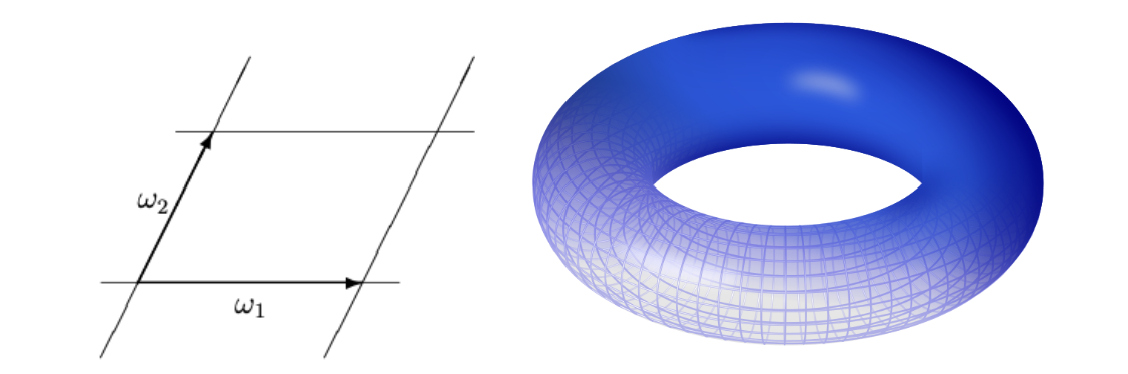
\includegraphics[width=0.8\textwidth]{img/torus_geometry.png}
    \caption{The torus is constructed by identifying points in the complex plane according to a lattice generated by two vectors \(\omega_1\) and \(\omega_2\). The fundamental domain is the parallelogram spanned by these vectors.}
\end{figure}
Because we are studying a Conformal Field Theory, global scale transformations and rotations are exact symmetries. Therefore, the physics cannot depend on the overall size or orientation of the lattice, but only on the ratio of the two vectors. We can completely characterize the conformal equivalence class of the torus by a single complex parameter:
\[
    \tau = \frac{\omega_2}{\omega_1}.
\]
We can always rotate the plane so that \(\omega_1\) lies along the positive real axis. To ensure the parallelogram does not degenerate and the orientation is standard, we require the imaginary part to be strictly positive: \(\mathrm{Im}(\tau) > 0\).

This \(\tau\) is called the \textbf{modular parameter}. Topologically, all tori are identical, but they are \textit{not} conformally equivalent. Tori with different values of \(\tau\) generally cannot be mapped into one another by conformal transformations.

However, the choice of the basis vectors \((\omega_1, \omega_2)\) for a given lattice \(\Lambda\) is highly non-unique. We can choose any other integer linear combination to generate the exact same lattice, provided the area of the fundamental parallelogram remains invariant. This corresponds to the matrix transformation:
\[
    \begin{pmatrix}
        \omega_1' \\
        \omega_2'
    \end{pmatrix} = \begin{pmatrix}
        a & b \\
        c & d
    \end{pmatrix} \begin{pmatrix}
        \omega_1 \\
        \omega_2
    \end{pmatrix}, \quad \text{with } a,b,c,d \in \mathbb{Z} \text{ and } \det\begin{pmatrix} a & b \\ c & d \end{pmatrix} = ad - bc = 1.
\]
This matrix belongs to the Special Linear group \(\mathrm{SL}(2, \mathbb{Z})\). Under this change of basis, the modular parameter transforms via a Möbius transformation:
\[
    \tau \to \tau' = \frac{a\tau + b}{c\tau + d}.
\]
Notice that flipping the signs of all coefficients (\(a,b,c,d \to -a,-b,-c,-d\)) leaves \(\tau'\) completely unchanged. Therefore, the true group of transformations on \(\tau\) is the projective group \(\mathrm{PSL}(2, \mathbb{Z}) = \mathrm{SL}(2, \mathbb{Z}) / \mathbb{Z}_2\). This is the \textbf{Modular Group}.

The entire modular group is generated by just two fundamental transformations:
\begin{itemize}
    \item \textbf{The \(\mathcal{T}\) transformation:} \(\tau \to \tau + 1\). This corresponds physically to a Dehn twist (cutting the torus, twisting one end by a full circle, and gluing it back).
    \item \textbf{The \(\mathcal{S}\) transformation:} \(\tau \to -1/\tau\). This corresponds to swapping the roles of the spatial cycle and the temporal cycle (interchanging \(\omega_1\) and \(\omega_2\)).
\end{itemize}
In matrix representation, they are:
\[
    \mathcal{T} = \begin{pmatrix} 1 & 1 \\ 0 & 1 \end{pmatrix}, \quad \mathcal{S} = \begin{pmatrix} 0 & 1 \\ -1 & 0 \end{pmatrix},
\]
and they satisfy the fundamental algebraic constraints:
\[
    \mathcal{S}^2 = \mathbb{I}, \quad (\mathcal{S}\mathcal{T})^3 = \mathbb{I}.
\]
The principle of modular invariance states that since \(\tau\) and \(\tau'\) describe the exact same physical torus (just parameterized differently), \uline{any physical observable lacking boundary insertions (most importantly, the partition function) must be strictly invariant under the generators \(\mathcal{S}\) and \(\mathcal{T}\)}.

\subsection{CFT on the Torus}

To compute the partition function, we first map the complex plane into a cylinder along the \(\omega_1\) direction. Assuming \(\omega_1\) lies along the real axis, the conformal map is:
\[
    z = e^{\frac{2\pi i}{\omega_1}w}.
\]
On this cylinder, the Hamiltonian (which generates Euclidean time translations) and the momentum operator (which generates spatial translations) are expressed in terms of the Virasoro zero-modes:
\[
    H = \frac{2\pi}{\omega_1} \left( L_0 + \bar{L}_0 - \frac{c}{12} \right), \quad P = \frac{2\pi}{\omega_1} \left( L_0 - \bar{L}_0 \right).
\]

To form the torus, we evolve the system along the cylinder and then glue the ends. The displacement vector closing the torus is \(\omega_2\). This displacement consists of an Euclidean time evolution of length \(\mathrm{Im}(\omega_2)\), combined with a spatial translation (a twist) of length \(\mathrm{Re}(\omega_2)\). The corresponding transfer matrix operator is:
\[
    \hat{T} = e^{-H \mathrm{Im}(\omega_2) + i P \mathrm{Re}(\omega_2)}.
\]
Substituting the expressions for \(H\) and \(P\), and using \(\mathrm{Im}(\omega_2) = \frac{\omega_2 - \bar{\omega}_2}{2i}\) and \(\mathrm{Re}(\omega_2) = \frac{\omega_2 + \bar{\omega}_2}{2}\), the exponent becomes:
\[
    i\pi \frac{\omega_2 - \bar{\omega}_2}{\omega_1} \left( L_0 + \bar{L}_0 - \frac{c}{12} \right) + i\pi \frac{\omega_2 + \bar{\omega}_2}{\omega_1} \left( L_0 - \bar{L}_0 \right).
\]
By grouping the holomorphic (\(L_0\)) and anti-holomorphic (\(\bar{L}_0\)) terms and using \(\tau = \omega_2/\omega_1\), this simplifies beautifully to:
\[
    \hat{T} = e^{2\pi i \tau \left(L_0 - \frac{c}{24}\right)} e^{-2\pi i \bar{\tau} \left(\bar{L}_0 - \frac{c}{24}\right)}.
\]

\subsubsection{Partition Function}

To impose periodic boundary conditions after this \(\omega_2\) translation and close the torus, we take the trace of the transfer matrix over the entire physical Hilbert space \(\mathcal{H}\) of the CFT:
\[
    Z(\tau, \bar{\tau}) \mapsto Z(q, \bar{q}) = \mathrm{Tr}_{\mathcal{H}} \hat{T} = \mathrm{Tr}_{\mathcal{H}} \left[ q^{L_0 - \frac{c}{24}} \bar{q}^{\bar{L}_0 - \frac{c}{24}} \right],
\]
where we have introduced the standard modular parameters:
\[
    q = e^{2\pi i \tau}, \quad \bar{q} = e^{-2\pi i \bar{\tau}}.
\]

As we have seen extensively, the Hilbert space of a 2D CFT is organized as a direct sum of irreducible highest-weight representations (Verma modules modulo null states) of the left and right Virasoro algebras:
\[
    \mathcal{H}_c = \bigoplus_{h, \bar{h}} \mathcal{N}_{h,\bar{h}} \, \mathcal{V}_{c,h} \otimes \mathcal{V}_{c,\bar{h}}.
\]
Because the trace is a linear operator, it perfectly factorizes over this direct sum:
\[
    Z(q, \bar{q}) = \sum_{h, \bar{h}} \mathcal{N}_{h,\bar{h}} \, \mathrm{Tr}_{\mathcal{V}_{c,h}} \left[ q^{L_0 - \frac{c}{24}} \right] \cdot \mathrm{Tr}_{\mathcal{V}_{c,\bar{h}}} \left[ \bar{q}^{\bar{L}_0 - \frac{c}{24}} \right].
\]
We can rewrite the partition function entirely as a sum over the \textbf{characters} \(\chi_h(q) \equiv \chi_h(\tau)\) of these irreducible representations:
\[
    Z(\tau, \bar{\tau}) = \sum_{h, \bar{h}} \mathcal{N}_{h,\bar{h}} \chi_h(\tau) \bar{\chi}_{\bar{h}}(\bar{\tau}).
\]
This shows that the partition function is a \textit{sesquilinear form} in the characters of the irreducible Virasoro representations composing the theory.

The role of the partition function is to meticulously count the states in the Hilbert space. Thanks to the state-operator correspondence, it perfectly describes the complete operator content of the theory:
\begin{itemize}
    \item The non-negative integer \(\mathcal{N}_{h,\bar{h}}\) gives the exact multiplicity of each conformal family.
    \item The exponents of the leading terms of \(q\) and \(\bar{q}\) give the conformal dimensions \((h, \bar{h})\) of the primary fields.
\end{itemize}

In the end we obtain a compact formula for the partition function, which encodes the entire operator content of the theory in a single mathematical object:
\[
    Z(q, \bar{q}) = (q \bar{q})^{-\frac{c}{24}} \sum_{h, \bar{h}} \mathcal{N}_{h,\bar{h}} q^h \bar{q}^{\bar{h}} \sum_{N, \bar{N}=0}^\infty a_N q^N \cdot \bar{a}_{\bar{N}} \bar{q}^{\bar{N}}.
\]
The coefficients \(a_N, \bar{a}_{\bar{N}}\) in the Taylor expansion of the characters give the dimensionalities of the secondary descendant levels.

\begin{example}[The Ising Partition Function]
    For the critical Ising model (\(c = 1/2\)), we found three primary fields: \(\mathbb{I} \, (h=0)\), \(\sigma \, (h=1/16)\), and \(\varepsilon \, (h=1/2)\). The requirement of modular invariance rigidly fixes their multiplicities \(\mathcal{N}_{h,\bar{h}}\) to be exactly 1 for the scalar combinations, and 0 otherwise. Thus, the physical partition function is exactly:
    \[
        Z_{\mathrm{Ising}}(\tau) = |\chi_0(\tau)|^2 + |\chi_{1/16}(\tau)|^2 + |\chi_{1/2}(\tau)|^2.
    \]
    This confirms the operator content of the theory:
    \[
        \mathcal{A}_{\mathrm{Ising}} = [0,0] \oplus \left[\frac{1}{16}, \frac{1}{16}\right] \oplus \left[\frac{1}{2}, \frac{1}{2}\right] = [\mathbb{I}] \oplus [\sigma] \oplus [\varepsilon].
    \]
\end{example}

\subsubsection{Modular Transformations of Characters}

To guarantee that \(Z(\tau, \bar{\tau})\) is modular invariant, we must understand how the individual characters \(\chi_h(\tau)\) behave under the \(\mathcal{S}\) and \(\mathcal{T}\) transformations.

For the \(\mathcal{T}\) transformation (\(\tau \to \tau + 1\)), the action is trivial. Remembering the general form of a character \(\chi_h(\tau) = q^{h - c/24} \sum a_n q^n\), shifting \(\tau \to \tau+1\) corresponds to multiplying \(q\) by \(e^{2\pi i} = 1\). The only phase picked up comes from the fractional exponent:
\[
    \mathcal{T} \,:\, \chi_h(\tau + 1) = e^{2\pi i \left(h - \frac{c}{24}\right)} \chi_h(\tau).
\]
This simply multiplies the characters by a constant phase matrix, which easily cancels out in \(Z(\tau, \bar{\tau})\) for scalar fields where \(h = \bar{h}\) (since \(e^{2\pi i(h-c/24)} e^{-2\pi i(h-c/24)} = 1\)).

The \(\mathcal{S}\) transformation (\(\tau \to -1/\tau\)) is far more involved. Computing it requires a heavy analytical tool known as the \textbf{Poisson Resummation Formula}. This is a profound mathematical identity relating an infinite series of a function to an infinite series of its Fourier transform:
\[
    \sum_{n \in \mathbb{Z}} G(x + nT_0) = \frac{1}{T_0} \sum_{k \in \mathbb{Z}} \tilde{G}\left(\frac{2\pi k}{T_0}\right) e^{\frac{2\pi i k x}{T_0}},
\]
where \(\tilde{G}(p) = \int_{-\infty}^{+\infty} G(x)e^{-ipx}\mathrm{d}x\). A heuristic physics proof (allowing for the use of distributions) relies on the Dirac comb identity in distribution theory: $\sum \delta(x - nT) = \frac{1}{T} \sum e^{2\pi i k x / T}$.

By applying this resummation formula to the explicit Theta-function representations of the minimal model characters (the Rocha-Caridi formulas), one can rigorously prove that under \(\tau \to -1/\tau\), the character of a specific primary field \((r,s)\) transforms into a \textit{linear combination} of all the other characters in the Kac table:
\[
    \mathcal{S} \,:\, \chi_{r,s}\left(-\frac{1}{\tau}\right) = \sum_{r',s'} \mathcal{S}_{r,s}^{r',s'} \chi_{r',s'}(\tau).
\]
The modular \(\mathcal{S}\)-matrix \(\mathcal{S}_{r,s}^{r',s'}\) is symmetric, unitary, and exactly calculable. For the unitary minimal models \(\mathcal{M}_m\), its entries are given by:
\[
    \mathcal{S}_{r,s}^{r',s'} = (-1)^{(r+s)(r'+s')} \sqrt{\frac{8}{m(m+1)}} \sin\left( \frac{\pi r r'}{m} \right) \sin\left( \frac{\pi s s'}{m+1} \right).
\]
The requirement that the sesquilinear sum \(Z = \sum \mathcal{N}_{h,\bar{h}} \chi_h \bar{\chi}_{\bar{h}}\) remains invariant under this intricate linear mixing imposes devastatingly strong constraints on the allowed multiplicities \(\mathcal{N}_{h,\bar{h}}\). Solving these matrix constraints is what led to the ADE classification (A-D-E Dynkin diagrams) of all possible modular invariant partition functions for minimal models, representing the crowning achievement of the classification program in two-dimensional CFT.

\section{Modular Invariance}

Modular invariance is a profoundly powerful macroscopic constraint on the structure of conformal field theories defined on the torus. It allows us to rigorously classify the minimal models and understand their properties in a systematic way. The core idea is that since the physical partition function $Z(\tau, \bar{\tau})$ counts the states of the system, it must be completely independent of the arbitrary choice of the basis vectors used to parameterize the torus. We can impose this geometric invariance to obtain severe algebraic constraints on the spectrum of the theory and the structure of the Virasoro representations.

\subsection{Constraints from Modular Invariance}

The partition function is written as a sesquilinear sum of characters, which are functions of the modular parameters $\tau$ and $\bar{\tau}$. To guarantee modular invariance, we require:
\[
    Z(\tau, \bar{\tau}) = Z\left(\frac{a\tau + b}{c\tau + d}, \frac{a\bar{\tau} + b}{c\bar{\tau} + d}\right).
\]
This is completely achieved if the partition function is strictly invariant under the two fundamental generators of the modular group, $\mathcal{S}$ and $\mathcal{T}$. These invariances will give us rigorous \textbf{Diophantine equations} for the coefficients $\mathcal{N}_{h,\bar{h}}$ that appear in the sum. These non-negative integers count the multiplicity of the representations with conformal weights $(h, \bar{h})$ in the physical spectrum of the theory. By solving these equations, we can determine the exact operator content of the theory, and consequently compute the critical exponents and other physical properties.

\subsubsection{The $\mathcal{T}$ Constraint}

The $\mathcal{T}$ transformation corresponds to a Dehn twist: $\tau \to \tau + 1$. We demand:
\[
    Z(\tau + 1, \bar{\tau} + 1) = Z(\tau, \bar{\tau}).
\]

We know the general partition function takes the form:
\[
    Z(\tau, \bar{\tau}) = \sum_{h,\bar{h}} \mathcal{N}_{h,\bar{h}}\chi_h(\tau)\chi_{\bar{h}}(\bar{\tau}).
\]
Evaluating the characters under this shift, we use the property $q \to q e^{2\pi i}$. The character transforms as:
\[
    \chi_h (\tau+1) = \mathrm{Tr}_{\mathcal{V}_{c,h}} \left( q^{L_0 - \frac{c}{24}} e^{2\pi i \left(L_0 - \frac{c}{24}\right)} \right).
\]
Because the eigenvalues of $L_0$ are $h + n$ with $n \in \mathbb{N}$, the integer shift $e^{2\pi i n} = 1$ factors out completely, and the character simply picks up a global phase from the ground state:
\[
    \chi_h (\tau+1) = e^{2 \pi i \left(h - \frac{c}{24}\right)} \chi_h(\tau).
\]

Inserting this transformation back into the expression for the partition function, we obtain:
\[
    Z(\tau+1, \bar{\tau}+1) = \sum_{h, \bar{h}} \mathcal{N}_{h,\bar{h}} e^{2 \pi i \left(h - \frac{c}{24}\right)} e^{-2 \pi i \left(\bar{h} - \frac{c}{24}\right)} \chi_h(\tau)\chi_{\bar{h}}(\bar{\tau}).
\]
For this to strictly equal $Z(\tau, \bar{\tau})$, the overall phase multiplying each non-zero term must be exactly 1. The Casimir energy terms ($c/24$) magically cancel out, leaving the constraint:
\[
    e^{2\pi i (h - \bar{h})} = 1 \quad \implies \quad s = h - \bar{h} \in \mathbb{Z}.
\]
\uline{This proves that strict modular invariance on the torus admits only primary fields with integer conformal spin.} By enforcing strictly periodic boundary conditions in both the $\omega_1$ and $\omega_2$ directions, we geometrically isolate the purely \textbf{bosonic sector} of the theory.

For example, in the Ising model, the composite energy density $\varepsilon = \psi\bar{\psi}$ (spin 0) is allowed, but the isolated Majorana fermions $\psi$ and $\bar{\psi}$ (spin $\pm 1/2$) are mathematically forbidden in this specific partition function. If we want to include and count fermions properly, we must release the requirement of full $\mathrm{PSL}(2,\mathbb{Z})$ invariance and restrict ourselves to the modular subgroup \(\Gamma(2) = \mathrm{PSL}(2,\mathbb{Z})/\mathbb{Z}_{2}\), which requires invariance only under $\tau \to \tau + 2$. This geometric relaxation allows for \textit{antiperiodic} boundary conditions (Spin Structures) where the fermions pick up a minus sign upon wrapping the torus.

\subsubsection{The $\mathcal{S}$ Constraint}

We now consider the $\mathcal{S}$ transformation, $\tau \to -1/\tau$, corresponding to the exchange of the spatial and temporal cycles of the torus:
\[
    Z\left(-\frac{1}{\tau}, -\frac{1}{\bar{\tau}}\right) = Z(\tau, \bar{\tau}).
\]

To express the new characters in terms of the old ones, as we have seen, we rely on the Poisson Resummation Formula, reported for clarity. Given a sufficiently well-behaved function $G(x)$, the formula states:
\[
    \sum_{n \in \mathbb{Z}} G(x + n T) = \frac{1}{T} \sum_{k \in \mathbb{Z}} \tilde{G}\left(\frac{2 \pi k}{T}\right)e^{\frac{2 \pi i}{T}kx},
\]
where $\tilde{G}(p)$ is the Fourier transform of $G(x)$.

By applying this advanced resummation to the exact character formulas, Cardy demonstrated that the characters under $\mathcal{S}$ transform linearly amongst themselves:
\[
    \chi_h\left(-\frac{1}{\tau}\right) = \sum_{h'} \mathcal{S}_{h, h'} \chi_{h'}(\tau).
\]
For minimal models, the modular $\mathcal{S}$-matrix is symmetric and unitary, explicitly given by:
\[
    \mathcal{S}_{(r,s), (r',s')} = (-1)^{(r+s)(r'+s')} \sqrt{\frac{8}{m(m+1)}} \sin \left( \frac{\pi r r'}{m} \right) \sin \left( \frac{\pi s s'}{m+1} \right).
\]

Substituting this linear transformation back into the partition function yields:
\[
    Z\left(-\frac{1}{\tau}, -\frac{1}{\bar{\tau}}\right) = \sum_{h, \bar{h}} \mathcal{N}_{h,\bar{h}} \left( \sum_{h'} \mathcal{S}_{h, h'} \chi_{h'}(\tau) \right) \left( \sum_{\bar{h}'} \mathcal{S}_{\bar{h}, \bar{h}'}^* \chi_{\bar{h}'}(\bar{\tau}) \right).
\]
By swapping the dummy indices and equating this to the original partition function $Z(\tau, \bar{\tau})$, we obtain a rigid algebraic constraint on the multiplicity coefficients:
\[
    \mathcal{N}_{h, \bar{h}} = \sum_{h', \bar{h}'} \mathcal{S}_{h, h'}^\dagger \mathcal{N}_{h', \bar{h}'} \mathcal{S}_{\bar{h}', \bar{h}}.
\]
This is a highly non-trivial constraint. Cardy recognized that these must be treated strictly as \textbf{Diophantine equations}, since the physical multiplicities $\mathcal{N}_{h,\bar{h}}$ must be non-negative integers ($\in \mathbb{N}_0$), and uniqueness of the vacuum dictates $\mathcal{N}_{0,0} = 1$. Solving these matrix constraints is what fundamentally restricts the landscape of CFTs and classifies the minimal models.

\subsection{Unitary Representations of the Modular Group}

We can compactly package these constraints using matrix notation. Let us collect all the characters of the Kac table into a column vector $\chi(\tau)$, and its conjugate transpose into a row vector $\chi^\dagger(\bar{\tau})$
\[
    \chi(\tau) = \begin{pmatrix}
        \chi_{0}(\tau) \\
        \vdots         \\
        \chi_{h}(\tau) \\
        \vdots
    \end{pmatrix}, \quad \chi^\dagger(\bar{\tau}) = \begin{pmatrix}
        \bar{\chi}_{0}(\bar{\tau}) & \cdots & \bar{\chi}_{\bar{h}}(\bar{\tau}) & \cdots
    \end{pmatrix}.
\]
The multiplicities form a square matrix $\mathcal{N}$ of non-negative integers. The partition function is simply the bilinear form:
\[
    Z(\tau, \bar{\tau}) = \chi^\dagger(\bar{\tau}) \mathcal{N} \chi(\tau).
\]

The modular transformations act as unitary matrices $\mathcal{T}$ (diagonal, with entries $e^{2\pi i(h - c/24)}$) and $\mathcal{S}$ acting on the vector $\chi$. The requirement of modular invariance translates to:
\[
    \mathcal{T}^\dagger \mathcal{N} \mathcal{T} = \mathcal{N}, \quad \text{and} \quad \mathcal{S}^\dagger \mathcal{N} \mathcal{S} = \mathcal{N}.
\]
Equivalently, since $\mathcal{S}$ and $\mathcal{T}$ are unitary, the physical multiplicity matrix $\mathcal{N}$ must commute with the modular generators:
\[
    [\mathcal{N}, \mathcal{T}] = 0, \quad \text{and} \quad [\mathcal{N}, \mathcal{S}] = 0.
\]
Finding all possible integer matrices $\mathcal{N}$ that commute with both $\mathcal{S}$ and $\mathcal{T}$ completes the ADE classification of minimal models.

\subsection{Classification of Minimal Models}

\subsubsection{The Diagonal Solution}

The most obvious, trivial solution to the matrix commutation equations is simply the identity matrix: $\mathcal{N} = \mathbb{I}$, meaning $\mathcal{N}_{h,\bar{h}} = \delta_{h,\bar{h}}$.

This universally valid solution is called the \textbf{diagonal modular invariant}. In this configuration, only scalar fields (where the left and right conformal weights are strictly identical, $h = \bar{h}$) physically appear in the spectrum, and each appears exactly once. The partition function takes the simple form:
\[
    Z_{\mathrm{diag}}(\tau) = \frac{1}{K} \sum_{h} \vert \chi_h(\tau) \vert^2,
\]
where $K$ is a normalization constant that can be fixed by demanding $\mathcal{N}_{0,0} = 1$ (uniqueness of the vacuum). This diagonal solution corresponds to the most basic universality class of the minimal model, and it is the one most commonly encountered in statistical mechanics. However, as we will see, it is not the only possible solution at higher central charges.

\begin{example}[Ising Model ($\mathcal{M}_3$)]
    For the critical Ising model ($c=1/2$), the diagonal solution is the unique, definitive solution. The partition function is:
    \[
        Z_{\mathrm{Ising}}(\tau) = \vert \chi_{0}(\tau) \vert^2 + \vert \chi_{\frac{1}{16}}(\tau) \vert^2 + \vert \chi_{\frac{1}{2}}(\tau) \vert^2.
    \]
    There are no other mathematically valid solutions to the Diophantine equations for $c=1/2$. This proves that the Ising universality class is the \textit{only} strictly unitary CFT sitting at this central charge, and this is its bosonic sector in the algebra of local fields.
\end{example}

\begin{example}[Tricritical Ising Model ($\mathcal{M}_4$)]
    For $m=4$ ($c=7/10$), the diagonal solution corresponds to the tricritical Ising model. The Kac table dictates six distinct scalar primary fields:
    \[
        Z_{\mathrm{Tricritical}} = \vert \chi_{0} \vert^2 + \vert \chi_{\frac{3}{80}} \vert^2 + \vert \chi_{\frac{1}{10}} \vert^2 + \vert \chi_{\frac{7}{16}} \vert^2 + \vert \chi_{\frac{3}{5}} \vert^2 + \vert \chi_{\frac{3}{2}} \vert^2.
    \]
    Again, this is the uniquely allowed physical modular invariant at $c=7/10$.
\end{example}

\subsubsection{Non-Diagonal Solutions and Extended Symmetries ($\mathcal{M}_5$)}

As we move up the minimal series, the Diophantine equations suddenly permit multiple, distinct mathematical solutions at the same central charge, representing entirely different universality classes.

For $\mathcal{M}_5$ ($c=4/5$), there is the standard \textbf{diagonal modular invariant} containing 10 scalar terms:
\[
    Z_{\mathrm{RSOS}_5} = |\chi_0|^2 + |\chi_{2/5}|^2 + |\chi_{7/5}|^2 + |\chi_{3}|^2 + |\chi_{1/8}|^2 + |\chi_{1/48}|^2 + |\chi_{21/48}|^2 + |\chi_{13/8}|^2 + |\chi_{2/3}|^2 + |\chi_{1/15}|^2.
\]
This describes a multicritical restricted solid-on-solid (RSOS) lattice model featuring a $\mathbb{Z}_2$ symmetry (it consists of two decoupled copies of the tricritical Ising model). The operator content is purely bosonic, and there are no higher-spin conserved currents.

However, Cardy discovered a radically different \textbf{non-diagonal solution} for $c=4/5$:
\[
    Z_{\mathrm{3-Potts}} = \vert \chi_0 + \chi_3 \vert^2 + \vert \chi_{\frac{2}{5}} + \chi_{\frac{7}{5}} \vert^2 + 2\vert \chi_{\frac{1}{15}} \vert^2 + 2\vert \chi_{\frac{2}{3}} \vert^2.
\]
This describes the universality class of the \textbf{3-state Potts model}, which possesses an enhanced $\mathbb{Z}_3$ macroscopic symmetry.

The notation $\vert \chi_0 + \chi_3 \vert^2$ is incredibly revealing. It implies that the vacuum identity field ($h=0$) is inextricably paired with a field of spin $3$ ($h=3$). A primary field with integer spin \(s\geq 2\) physically corresponds to a \textbf{higher-spin conserved current} (specifically, the fields $W(z)$ and $\bar{W}(\bar{z})$).

The presence of this conserved current physically extends the local conformal symmetry. The fundamental symmetry algebra of the 3-state Potts model is not merely the standard Virasoro algebra, but rather a much larger \textbf{extended chiral algebra} known as the $\mathcal{W}_3$-algebra. This non-diagonal solution elegantly demonstrates how modular invariance on the torus natively detects and enforces the existence of higher hidden symmetries in statistical mechanics.

\section{Boundary Conditions and Invariants}

So far, in our construction of the partition function on the torus, we have implicitly assumed strictly periodic boundary conditions in both the spatial (\(\omega_1\)) and temporal (\(\omega_2\)) directions. This completely periodic configuration is conventionally denoted as \(Z_{1,1}\).

However, if the conformal field theory possesses a discrete global symmetry group \(G\), we can construct new, highly non-trivial partition functions by imposing \textbf{twisted boundary conditions}. For any two elements \(g, h \in G\), we can define a partition function \(Z_{g,h}\), where the first index refers to the twist along the \(\omega_1\) cycle, and the second refers to the twist along the \(\omega_2\) cycle.

Because \(G\) represents an exact symmetry of the model, its group elements act as operators \(\hat{g}\) that strictly commute with the Hamiltonian: \([H, \hat{g}] = 0\). This means they are simultaneously diagonalizable, and a basis of conformal states \(\ket{s}\) satisfies \(\hat{g}\ket{s} = g\ket{s}\). A twist in the ``time'' direction simply corresponds to inserting this symmetry operator inside the trace:
\[
    Z_{1,g}(\tau, \bar{\tau}) = \mathrm{Tr}_{\mathcal{H}} \left[ \hat{g} q^{L_0 - \frac{c}{24}} \bar{q}^{\bar{L}_0 - \frac{c}{24}} \right] = \sum_{\Delta, \bar{\Delta}} \mathcal{N}_{\Delta, \bar{\Delta}} \, g \, \chi_{\Delta}(\tau) \chi_{\bar{\Delta}}(\bar{\tau}).
\]

\begin{example}[Twisted Sectors in the Ising Model]
    In minimal models, there is always an inherent \(\mathbb{Z}_2 = \{+, -\}\) symmetry arising from the folding of the Kac table (physically reflecting the Kramers-Wannier duality). Let us impose an antiperiodic boundary condition (\(-\)) in the time direction for the Ising model. This introduces a parity sign \(P_{r,s}\) inside the sum:
    \[
        Z_{+,-} = \sum_{r,s,\bar{r},\bar{s}} \mathcal{N}_{\Delta \bar{\Delta}} P_{r,s} \bar{P}_{\bar{r},\bar{s}} \chi_{r,s} \chi_{\bar{r},\bar{s}}, \quad \text{where } P_{r,s} = \begin{cases} (-1)^r & m \text{ even} \\ (-1)^s & m \text{ odd} \end{cases}
    \]
    For the Ising model (\(m=3\), odd), the parity depends on \(s\). The resulting twisted partition function is:
    \[
        Z_{+,-} = |\chi_0|^2 - \left|\chi_{\frac{1}{16}}\right|^2 + \left|\chi_{\frac{1}{2}}\right|^2.
    \]
    Notice the minus sign! This function is \uline{not} modular invariant, nor does it represent a pure counting of states anymore, as the coefficients are not all non-negative integers.

    However, the proper counting property is restored if we apply the modular \(\mathcal{S}\)-transformation (\(\tau \to -1/\tau\)), which geometrically swaps the cycles, mapping \(Z_{1,g}\) into \(Z_{g,1}\) (a spatial twist). For the Ising model, exploring the fully antiperiodic sector (\(Z_{--}\)) isolates exactly the \(\mathbb{Z}_2\)-odd fermions:
    \[
        Z_{-,-} = -\chi_{\frac{1}{2}}\bar{\chi}_0 - \chi_0\bar{\chi}_{\frac{1}{2}} + \left|\chi_{\frac{1}{16}}\right|^2.
    \]
\end{example}

\subsection{Orbifold Theories}

While individual twisted sectors \(Z_{g,h}\) are not modular invariant on their own, one can form a perfectly valid, new modular invariant partition function by systematically summing up all possible boundary conditions over the entire symmetry group \(G\). This mathematical procedure of taking a quotient of the theory by a discrete symmetry is known as \textbf{Orbifolding}.

The orbifold partition function is defined as the group average:
\[
    Z_{\mathrm{orb}} = \frac{1}{|G|} \sum_{g,h \in G} Z_{g,h}.
\]

For the universal \(\mathbb{Z}_2\) symmetry present in minimal models, the orbifold partition function requires summing four distinct sectors:
\[
    Z_{\mathrm{orb}} = \frac{1}{2} \left( Z_{++} + Z_{+-} + Z_{-+} + Z_{--} \right).
\]
Fascinatingly, if we explicitly perform this sum for the Ising model (\(m=3\)), the minus signs perfectly cancel out the fermionic off-diagonal terms, and we miraculously recover exactly the diagonal partition function: \(Z_{\mathrm{orb}} = Z_{\mathrm{diag}}\). This proves that the critical Ising model is \textbf{self-dual} under \(\mathbb{Z}_2\) orbifolding.

\subsection{Modular Invariants in Minimal Models}

We have seen that one universal solution to the Diophantine equations implied by modular invariance is the \textbf{diagonal solution} (\(\mathcal{N}_{h,\bar{h}} = \delta_{h,\bar{h}}\)). However, the orbifold procedure guarantees that a second, \textbf{non-diagonal} solution can often be constructed. Let us systematically map out the complete landscape of unitary minimal models characterized by the central charge \(c = 1 - 6/(m(m+1))\).

\begin{itemize}
    \item \textbf{For \(m=3\) (Ising) and \(m=4\) (Tricritical Ising):}
          Doing the orbifold procedure yields \(Z_{\mathrm{orb}} = Z_{\mathrm{diag}}\). There are strictly no other solutions. These two models are uniquely defined by their diagonal invariants and are self-dual with respect to the \(\mathbb{Z}_2\) symmetry.

    \item \textbf{For \(m \ge 5\):}
          We always obtain at least two distinct modular invariants. The diagonal solution \(Z_{\mathrm{diag}}\) corresponds physically to Restricted Solid-on-Solid (RSOS) lattice models, whose ``spin'' variables take values on linear graphs. The non-diagonal orbifold solution \(Z_{\mathrm{orb}} \neq Z_{\mathrm{diag}}\) corresponds to a different universality class at the exact same central charge.

          In the specific case of \(m=5\) and \(m=6\), the orbifold invariant exhibits an enhanced \(\mathbb{Z}_3\) symmetry (like the 3-state Potts model we discussed earlier). For all other \(m \ge 7\), the enhanced symmetry is just the standard \(\mathbb{Z}_2\) Kramers-Wannier duality.

    \item \textbf{The Exceptional Solutions:}
          Remarkably, at very specific, isolated values of \(m\), entirely new and unexpected solutions to the Diophantine equations appear. These are called \textbf{exceptional invariants} (\(Z_{\mathrm{exc}}\)). They occur exactly at:
          \[
              m = 11, \, 12, \, 17, \, 18, \, 29, \, 30.
          \]
\end{itemize}

\subsubsection{The A-D-E Classification and Completeness}

The underlying mathematical structure unifying these diagonal, orbifold, and exceptional solutions is one of the most beautiful discoveries in mathematical physics. The allowed modular invariants are in perfect one-to-one correspondence with the simply-laced \textbf{Lie Algebras}, specifically the \textbf{A-D-E Dynkin diagrams}:
\begin{itemize}
    \item \textbf{A-series (\(A_m\)):} Corresponds to the \textit{diagonal} solutions (existing for all \(m \ge 3\)).
    \item \textbf{D-series (\(D_{m/2+1}\)):} Corresponds to the non-diagonal \textit{orbifold} solutions (existing for all \(m \ge 5\)).
    \item \textbf{E-series (\(E_6, E_7, E_8\)):} Corresponds exactly to the \textit{exceptional} solutions appearing at \(m=11,12\) (\(E_6\)), \(m=17,18\) (\(E_7\)), and \(m=29,30\) (\(E_8\)).
\end{itemize}

In 1986, A. Cappelli, C. Itzykson, and J.B. Zuber, using incredibly subtle properties of number theory encoded within theta functions, rigorously proved that \uline{this A-D-E classification is completely exhaustive}. There are absolutely no other unitary modular invariant partition functions for \(c < 1\).

\subsubsection{Conclusion}

This classification stands as one of the most important and monumental achievements in the history of two-dimensional Conformal Field Theory. We now possess a complete, rigorous, and absolutely exhaustive list of all possible unitary conformal field theories with a central charge between 0 and 1. These theories can be exactly solved, their entire operator content fully described, and their correlation functions explicitly calculated.

This definitive result opened the floodgates to modern theoretical physics. By knowing exactly the complete set of operators and their scaling dimensions, physicists can systematically select relevant operators to perturb the theory \textit{off} the critical point. This allows us to understand the physics not only exactly at phase transitions but also in their vicinities, paving the way for \textbf{Integrable Quantum Field Theories} and exact non-perturbative results. The rigorous machinery developed here continues to heavily influence advanced Statistical Mechanics, String Theory, Holography, and countless other frontiers of modern physics.